\documentclass[12pt]{article}
\usepackage{amsmath, amssymb, geometry, graphicx, hyperref, setspace, float, subcaption}

% Page settings
\geometry{a4paper, margin=1in}
\setlength{\parindent}{0pt}
\setlength{\parskip}{1em}
\onehalfspacing

% Title and author
\title{Assignment 1: Experiments and Analysis}
\author{Your Name}
\date{\today}

\begin{document}

% Title Page
\maketitle
\tableofcontents
\newpage

% Section 1: Introduction
\section{Introduction}
A binary classification was performed on a spam-email dataset from Spambase to determine whether an email was spam or not using multiple different statistical learning models. Models were implemented using SciKitLearn and numpy, and graphs were generated using MatPlotLib.


% Section 2: Results and Analysis
\section{Part I: Separate Analysis}
The separate analysis section includes the methods/models used and their individual performances. For each model, multiple approaches were taken in an attempt to determine the best ways to fit each model to this dataset.

\subsection{Decision Trees}

Decision trees were implemented in 4 different ways:

\begin{itemize}
    \item No pruning
    \item Minimum Cost-Complexity Pruning
    \item Reduced Error Pruning (Gini Index)
    \item Reduced Error Pruning (Just error as index)
\end{itemize}

In figure 1, you can see each of the decision trees after they have completely finished training. The pruned trees, of course, are considerable smaller than the non-pruned tree.

\begin{figure}[htbp]
    \centering
    % First row of graphs (2 graphs side by side)
    \begin{subfigure}{0.45\textwidth}
        \centering
        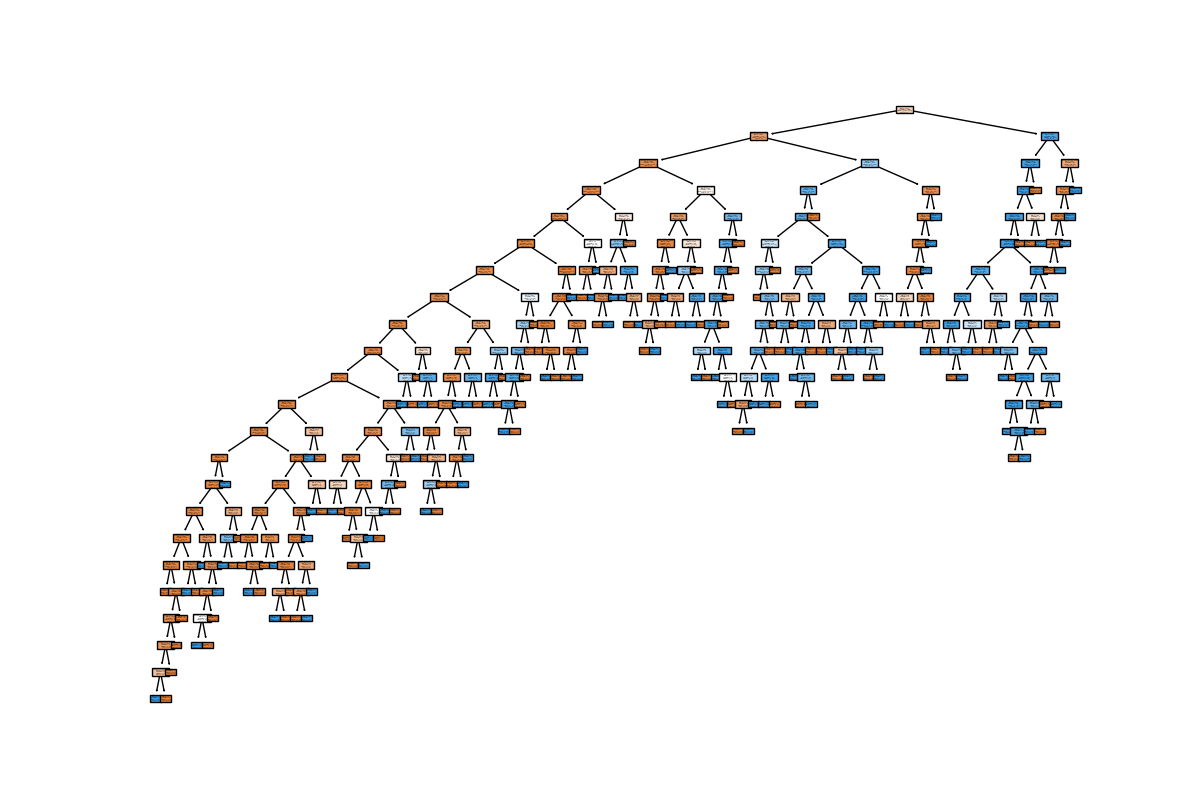
\includegraphics[width=\linewidth]{figures/Reduced Error Pruning/raw_tree.png}  % Replace with your image
        \caption{Raw Tree}
        \label{fig:method1}
    \end{subfigure}
    \hfill
    \begin{subfigure}{0.45\textwidth}
        \centering
        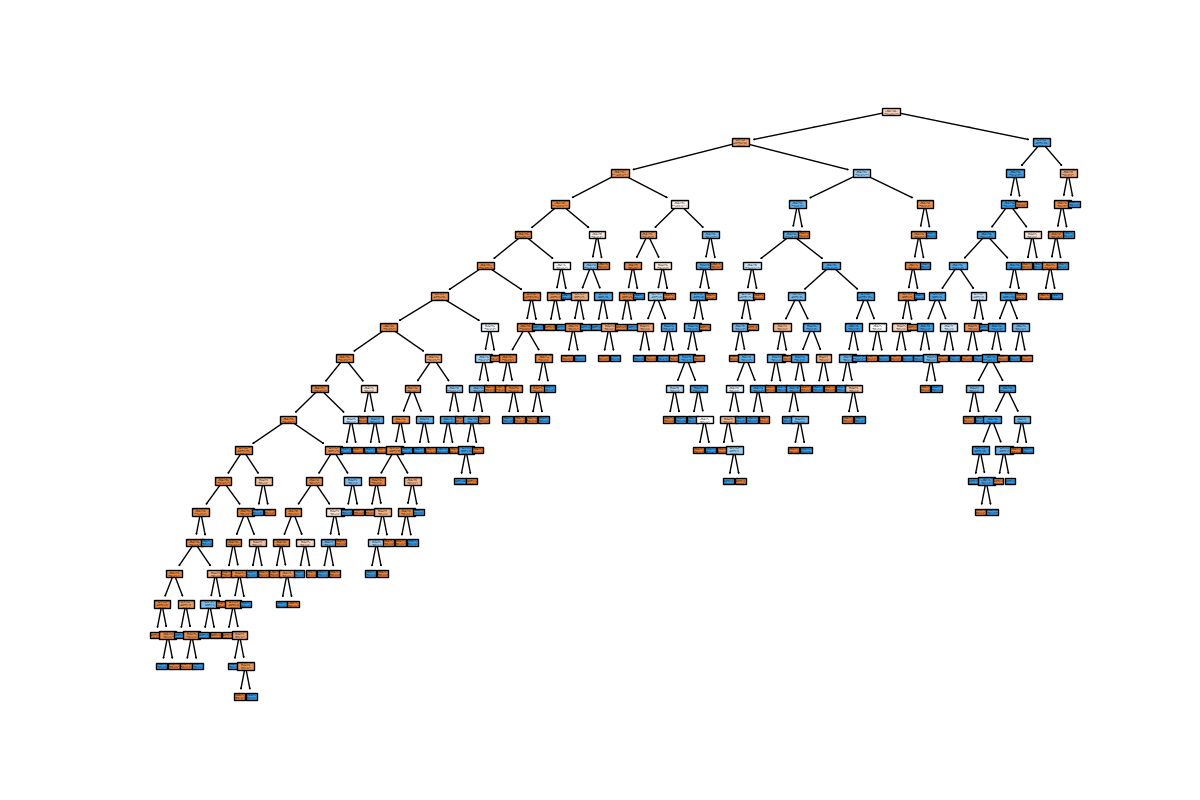
\includegraphics[width=\linewidth]{figures/Reduced Error Pruning/ccp tree.png}  % Replace with your image
        \caption{Cost-Complexity Pruning Tree}
        \label{fig:method2}
    \end{subfigure}
    
    % Second row of graphs (2 graphs side by side)
    \vskip\baselineskip  % Adds a line break between rows
    \begin{subfigure}{0.45\textwidth}
        \centering
        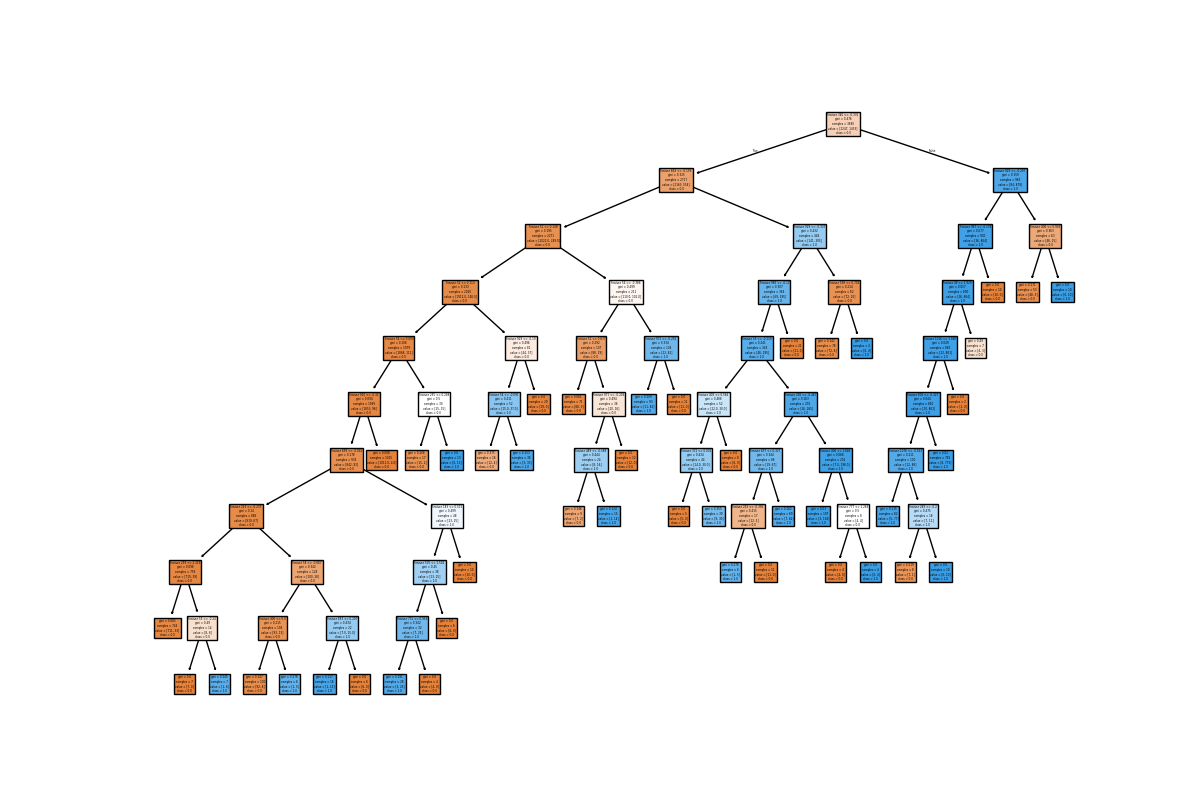
\includegraphics[width=\linewidth]{figures/Reduced Error Pruning/error_tree.png}  % Replace with your image
        \caption{Reduced Error Tree}
        \label{fig:method3}
    \end{subfigure}
    \hfill
    \begin{subfigure}{0.45\textwidth}
        \centering
        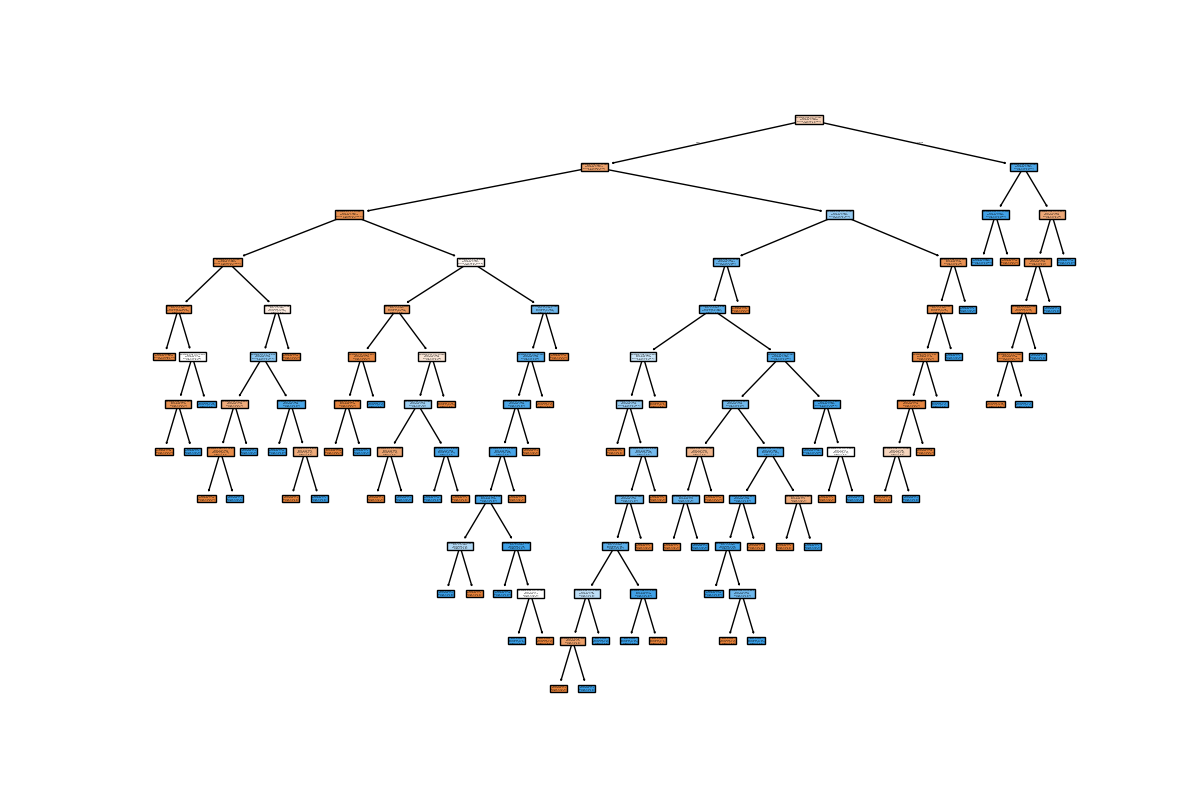
\includegraphics[width=\linewidth]{figures/Reduced Error Pruning/gini tree.png}  % Replace with your image
        \caption{Gini Index Tree}
        \label{fig:method4}
    \end{subfigure}

    \caption{Comparison of Different Training Methods}
    \label{fig:comparison}
\end{figure}


For each of the trees displayed in the figure, I used a cutoff value that made sure that they were pruned close to optimally. In order to find these cutoff values, I plotted the respective alphas of the pruning methods against the accuracies that implementing them produced.

\subsubsection{Minimum Cost-Complexity}

Here we can see the relationship between alpha and accuracy for Minimum Cost-Complexity Pruning:

\begin{figure}[h!]
    \centering
    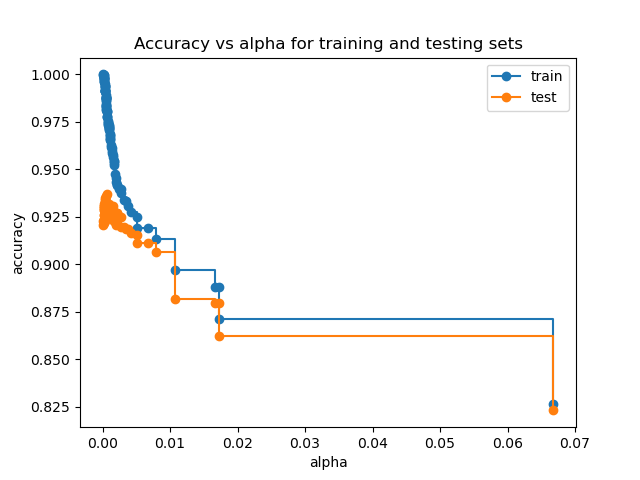
\includegraphics[width=0.8\linewidth]{figures/CCP/Accuracy vs alpha for train and test sets.png}
    \caption{Alpha vs. Accuracy for Minimum Cost-Complexity Pruning}
    \label{fig:mcc}
\end{figure}

\subsubsection{Reduced Error Pruning (Gini Index)}

Here we can see the relationship between alpha and accuracy for Reduced Error Pruning using the Gini Index:

\begin{figure}[h!]
    \centering
    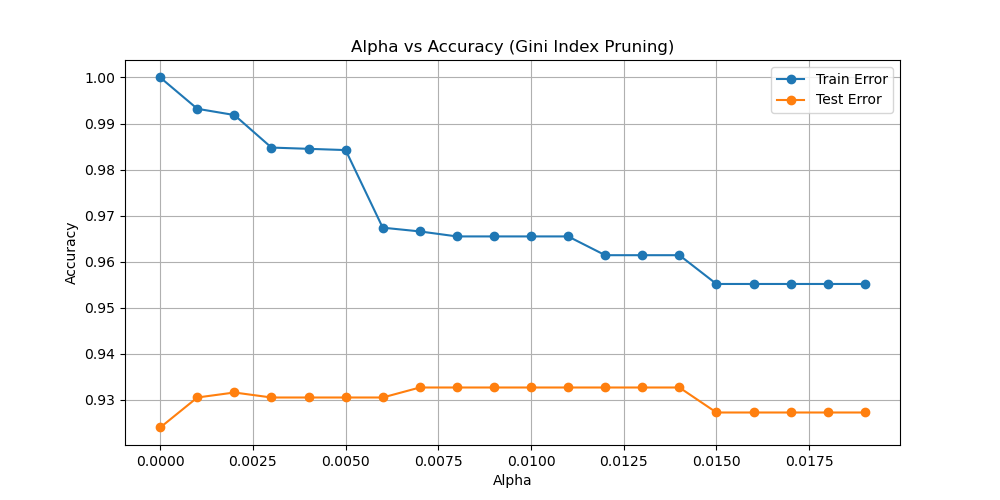
\includegraphics[width=0.8\linewidth]{figures/Reduced Error Pruning/gini alpha vs accuracy.png}
    \caption{Alpha vs. Accuracy for Reduced Error Pruning (Gini Index)}
    \label{fig:gini}
\end{figure}

\subsubsection{Reduced Error Pruning (Just Error)}

Here we can see the relationship between alpha and accuracy for Reduced Error Pruning using just error:

\begin{figure}[h!]
    \centering
    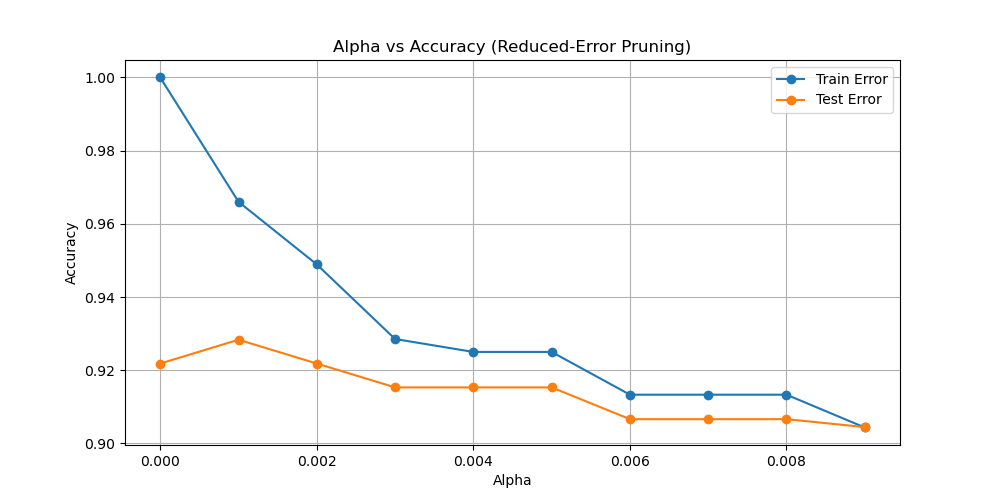
\includegraphics[width=0.8\linewidth]{figures/Reduced Error Pruning/alpha vs accuracy.png}
    \caption{Alpha vs. Accuracy for Reduced Error Pruning (Just Error)}
    \label{fig:error}
\end{figure}

\subsection{Random Forests}

To analyze random forests, I varied ensemble size and max depth and compared the error rates that they produced.

\begin{figure}[h!]
    \centering
    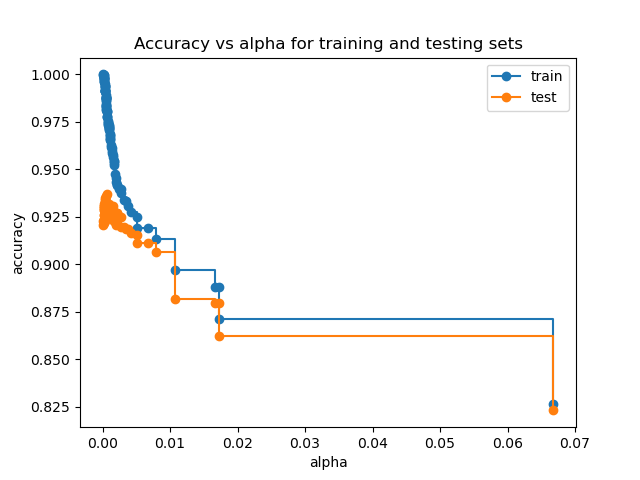
\includegraphics[width=0.8\linewidth]{figures/CCP/Accuracy vs alpha for train and test sets.png}
    \caption{Importance of Each Feature}
    \label{fig:mcc}
\end{figure}

\begin{figure}[h!]
    \centering
    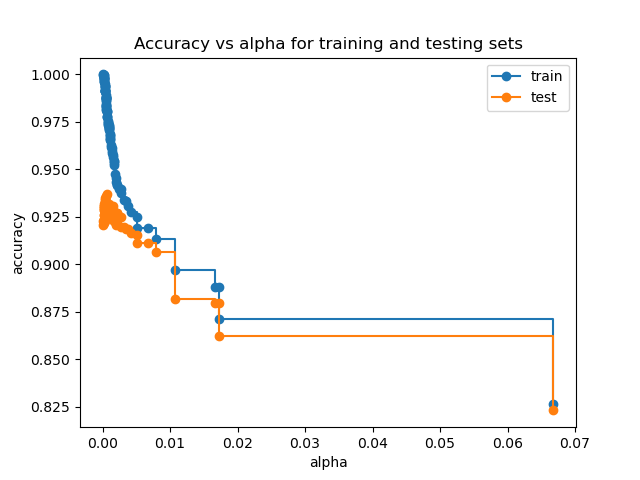
\includegraphics[width=0.8\linewidth]{figures/CCP/Accuracy vs alpha for train and test sets.png}
    \caption{Max depth vs training and test error rate}
    \label{fig:mcc}
\end{figure}

\begin{figure}[h!]
    \centering
    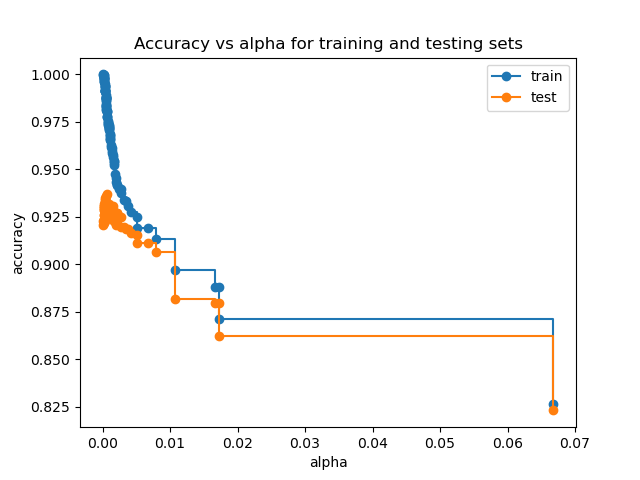
\includegraphics[width=0.8\linewidth]{figures/CCP/Accuracy vs alpha for train and test sets.png}
    \caption{Number of trees vs training and test error rate}
    \label{fig:mcc}
\end{figure}

\subsection{Boosted Decision Trees}
To analyze the AdaBoost decision tress, I varied the ensemble size and the weight of each stump and compared the error rates that they produced.

\section{Part II: Comparative Analysis}
Compare Random Forests and Boosted Decision Stumps:
\begin{itemize}
    \item Use k-fold cross-validation to tune the ensemble size for each method.
    \item Present results comparing test errors for the tuned versions of each method.
\end{itemize}

\newpage
% Section 4: Out-of-Bag Error Estimate
\section{Out-of-Bag Error Estimate}
Explain and present results for the OOB error estimate for Random Forests. Include:
\begin{itemize}
    \item Implementation details.
    \item Plot of OOB error vs. number of trees.
    \item Discussion of findings.
\end{itemize}

% Section 5: Conclusion
\section{Conclusion}
Summarize key findings from the analysis. Discuss strengths and weaknesses of the methods and potential improvements.

% Section 6: References
\section{References}
List any references used, including:
\begin{itemize}
    \item Dataset sources (e.g., UCI repository)
    \item Relevant libraries or documentation (e.g., scikit-learn)
\end{itemize}

% Section 7: Appendix
\appendix
\section{Appendix}
Include supplementary materials, additional plots, or code snippets if needed.

\end{document}
